\paragraph{QuizziPedia::Back-End::App::Models::QuizModel}
\label{QuizziPedia::Back-End::App::Models::QuizModel}
\begin{figure}[ht]
	\centering
	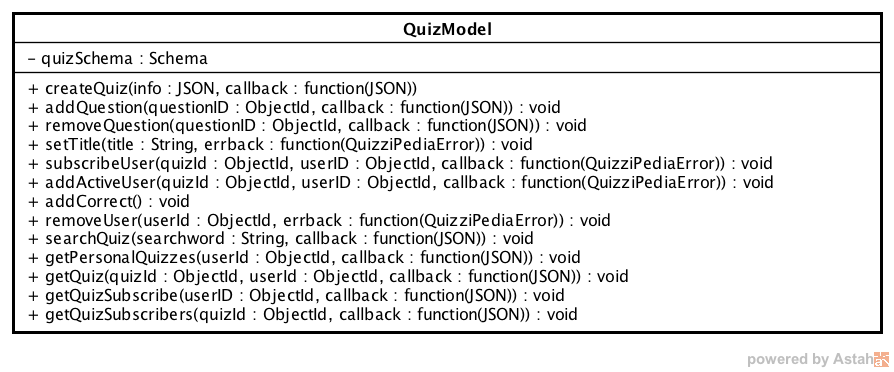
\includegraphics[scale=0.65]{UML/Classi/Back-End/QuizziPedia_Back-End_App_Models_quizModel.png}
	\caption{QuizziPedia::Back-End::App::Models::QuizModel}
\end{figure}
\FloatBarrier



\begin{itemize}
	\item \textbf{Descrizione}: classe che modella i questionari all'interno dell'applicazione;
	\item \textbf{Utilizzo}: viene utilizzata per rappresentare i dati relativi ai questionari all'interno dell'applicazione. Si interfaccia con la libreria \textit{Mongoose\ped{G}} per la creazione dello schema e dei relativi metodi statici o di istanza;
	\item \textbf{Relazioni con altre classi}:
		\begin{itemize}
			\item \textbf{OUT} \texttt{QuestionModel}\\
			Classe che rappresenta le operazioni relative alle domande;
			\item \textbf{OUT} \texttt{UserModel}\\
			Classe che rappresenta le operazioni relative agli utenti.
		\end{itemize}
	\item \textbf{Attributi}:
		\begin{itemize}
			\item \texttt{- quizSchema: Schema} \\
			Questo campo dati rappresenta lo schema \textit{Mongoose\ped{G}} dei quiz di \progetto. Lo schema prevede i seguenti attributi:
				\begin{itemize}
					\item \texttt{title: String}\\ Rappresenta il titolo del questionario;
					\item \texttt{author: ObjectId}\\ Rappresenta il riferimento all'identificativo nel database dell'utente che ha creato il questionario;
					\item \texttt{questions: Array<ObjectId>}\\ Array che contiene oggetti di tipo \texttt{ObjectId} che rappresentano i riferimenti agli identificativi nel database delle domande appartenenti al questionario;
					\item \texttt{registeredUsers: Array}\\ Array che contiene oggetti di tipo \texttt{ObjectId} che rappresentano i riferimenti agli identificativi nel database degli utenti iscritti al quiz;
					\item \texttt{activeUsers: Array}\\ Array che contiene oggetti di tipo \texttt{ObjectId} che rappresentano i riferimenti agli identificativi nel database degli utenti che partecipano effettivamente al questionario;
					\item \texttt{correctAnswers: Number}\\ Rappresenta il numero totale di risposte corrette date dagli utenti alle domande del questionario.	
				\end{itemize}
		\end{itemize}
	\item \textbf{Metodi}:
		\begin{itemize}
		
			\item \texttt{+ createQuiz(info: JSON, callback: function(JSON)): void}\\
			Crea un questionario con i dati che vengono passati.\\
			\textbf{Parametri}:
			\begin{itemize}
				\item \texttt{info: JSON}\\
				Rappresenta i dati del questionario che verrà creato;
				\item \texttt{callback: function(JSON)}\\
				Rappresenta la \textit{callback\ped{G}} che verrà eseguita al termine dell'elaborazione.
			\end{itemize}
			
			\item \texttt{+ addQuestion(questionID: ObjectId,  callback: function(JSON)): void}\\
			Aggiunge una domanda al questionario.\\
			\textbf{Parametri}:
			\begin{itemize}
				\item \texttt{questionID: ObjectId}\\
				Rappresenta l'identificativo della domanda da aggiungere al questionario;
				\item \texttt{callback: function(JSON)}\\
				Rappresenta la \textit{callback\ped{G}} che verrà eseguita al termine dell'elaborazione.
			\end{itemize}
			
			\item \texttt{+ removeQuestion(questionID: ObjectId, callback: function(JSON)): void}\\
			Rimuove una domanda dal questionario.\\
			\textbf{Parametri}:
			\begin{itemize}
				\item \texttt{questionID: ObjectId}\\
				Rappresenta l'identificativo della domanda da rimuovere dal questionario;
				\item \texttt{callback: function(JSON)}\\
				Rappresenta la \textit{callback\ped{G}} che verrà eseguita al termine dell'elaborazione.
			\end{itemize}
			
			\item \texttt{+ setTitle(title: String, callback: function(QuizziPediaError)): void}\\ 		
			Da un titolo al questionario.\\
			\textbf{Parametri}:
			\begin{itemize}
				\item \texttt{title: String}\\
				Rappresenta il titolo da dare al questionario;
				\item \texttt{callback: function(QuizziPediaError)}\\
				Rappresenta la \textit{callback\ped{G}} che verrà eseguita al termine dell'elaborazione in caso di errore.
			\end{itemize}
			
			\item \texttt{+ subscribeUser (quizId:ObjectId,userID: ObjectId, , callback: function(QuizziPediaError)): void}\\
			Aggiunge un utente dalla lista degli iscritti al questionario.\\
			\textbf{Parametri}:
			\begin{itemize}
				\item \texttt{quizId: ObjectId}\\
				Rappresenta l'identificativo del questionario a  cui aggiungere l'iscritto.
				\item \texttt{userID: ObjectId}\\
				Rappresenta l'identificativo dell'utente da aggiungere al questionario.
				\item \texttt{callback: function(QuizziPediaError)}\\
				Rappresenta la \textit{callback\ped{G}} che verrà eseguita al termine dell'elaborazione in caso di errore.
			\end{itemize}
			
			\item \texttt{+ addActiveUser(quizId: ObjectId, userID: ObjectId, callback: function(QuizziPediaError)): void}\\
			Aggiunge un utente dalla lista degli utenti che hanno svolto il questionario.\\
			\textbf{Parametri}:
			\begin{itemize}
				\item \texttt{quizId: ObjectId}\\
				Rappresenta l'identificativo del questionario a  cui aggiungere l'iscritto.
				\item \texttt{userID: ObjectId}\\
				Rappresenta l'identificativo dell'utente da aggiungere al questionario.
				\item \texttt{callback: function(QuizziPediaError)}\\
				Rappresenta la \textit{callback\ped{G}} che verrà eseguita al termine dell'elaborazione in caso di errore.
			\end{itemize}
			
			\item \texttt{+ addCorrect(): void}\\
			Incrementa il numero di risposte corrette date alle domande del questionario;		
			
			\item \texttt{+ removeUser(userID: ObjectId, \\callback: function(QuizziPediaError)): void}\\
			Rimuovere un utente dalla lista degli iscritti al questionario.\\
			\textbf{Parametri}:
			\begin{itemize}
				\item \texttt{userID: ObjectId}\\
				Rappresenta l'identificativo dell'utente da rimuovere dalla lista degli iscritti al questionario;
				\item \texttt{callback: function(QuizziPediaError)}\\
				Rappresenta la \textit{callback\ped{G}} che verrà eseguita al termine dell'elaborazione in caso di errore.
			\end{itemize}
			
			\item \texttt{+ searchQuiz(searchword: String, callback: function(JSON)): void}\\
			Ricerca un questionario.\\
			\textbf{Parametri}:
			\begin{itemize}
				\item \texttt{searchword: String}\\
				Rappresenta il titolo o l'autore del questionario da ricercare;
				\item \texttt{callback: function(JSON)}\\
				Rappresenta la \textit{callback\ped{G}} che verrà eseguita al termine dell'elaborazione;
			\end{itemize}
			
			\item \texttt{+ getPersonalQuizzes(userID: ObjectId, callback: function(JSON)): void}\\
			Ritorna i questionari creati da un utente pro.\\
			\textbf{Parametri}:
			\begin{itemize}
				\item \texttt{userID: ObjectId}\\
				Rappresenta l'identificativo dell'utente che ha creato i questionari che si vogliono ottenere;
				\item \texttt{callback: function(JSON)}\\
				Rappresenta la \textit{callback\ped{G}} che verrà eseguita al termine dell'elaborazione;
			\end{itemize}
			
			\item \texttt{+ getQuizSubscribe(userID: ObjectId,callback: function(JSON)): void}\\
				Ritorna i questionari ai quali l'utente si è iscritto.\\
				\textbf{Parametri}:
				\begin{itemize}
					\item \texttt{userID: ObjectId}\\
					Rappresenta l'identificativo dell'utente al quali si vogliono ritornare i questionari a cui si è iscritto;
					\item \texttt{callback: function(QuizziPediaError)}\\
					Rappresenta la \textit{callback\ped{G}} che verrà eseguita al termine dell'elaborazione in caso di errore.
				\end{itemize}
				
			\item \texttt{+ getQuizSubscribers(quizId: ObjectId,callback: function(JSON)): void}\\
			Ritorna gli iscritti ad un determinato questionario.\\
			\textbf{Parametri}:
			\begin{itemize}
				\item \texttt{quizId: ObjectId}\\
				Rappresenta l'identificativo del quiz al quale si vuole ritornare gli iscritti;
				\item \texttt{callback: function(QuizziPediaError)}\\
				Rappresenta la \textit{callback\ped{G}} che verrà eseguita al termine dell'elaborazione in caso di errore.
			\end{itemize}
				
			
			\item \texttt{+ getQuiz(quizId:ObjectId,userId:ObjectId,callback: function(JSON)): void}\\
			Ritorna il questionario da compilare.\\
			\textbf{Parametri}:
			\begin{itemize}
				\item \texttt{quizId: ObjectId}\\
				Rappresenta l'identificativo del quiz;
				\item \texttt{userId: ObjectId}\\
				Rappresenta l'identificativo dell'utente;
				\item \texttt{callback: function(JSON)}\\
				Rappresenta la \textit{callback\ped{G}} che verrà eseguita al termine dell'elaborazione.
			\end{itemize}
		\end{itemize}
\end{itemize}